\documentclass[11pt]{article}
\usepackage[margin=1in]{geometry}
\usepackage{booktabs}
\usepackage{array}
\usepackage{xcolor}
\usepackage{colortbl}
\usepackage{caption}
\usepackage{graphicx}
\usepackage{hyperref}
\usepackage{amsmath}
\usepackage{amssymb}
\usepackage{float}
\usepackage{enumitem}
\usepackage{fancyhdr}
\usepackage{subcaption}

\pagestyle{fancy}
\fancyhf{}
\rhead{ScaWL Replication --- \today}
\lhead{Stevens Lab}
\rfoot{\thepage}

\definecolor{darkgreen}{rgb}{0.0, 0.5, 0.0}
\definecolor{darkred}{rgb}{0.7, 0.0, 0.0}
\definecolor{paperblue}{rgb}{0.15, 0.35, 0.65}
\definecolor{oursred}{rgb}{0.8, 0.2, 0.2}

\newcommand{\paperval}[1]{\textcolor{paperblue}{#1}}
\newcommand{\ourval}[1]{\textcolor{oursred}{#1}}
\newcommand{\good}{\textcolor{darkgreen}{\checkmark}}
\newcommand{\bad}{\textcolor{darkred}{$\times$}}

\title{\textbf{Replication Report}\\[0.3em]
\large ScaWL: Scaling k-WL (Weisfeiler--Lehman) Algorithms in Distributed-Memory\\[0.3em]
\normalsize C.~Soss \emph{et al.}\\
\normalsize OSTI ID: 2587225}
\author{Replicator: Ollie (OpenClaw) \quad PI: Rick Stevens, Argonne National Laboratory}
\date{\today}

\begin{document}
\maketitle
\thispagestyle{fancy}

\section*{Executive Summary}
\begin{itemize}[leftmargin=1.5em,itemsep=2pt]
  \item \textbf{Domain:} graph algorithms / parallel computing. 2-dimensional Weisfeiler--Lehman color refinement as a graph-isomorphism invariant.
  \item \textbf{Scope of replication:} independent Python/NumPy re-implementation of 2-WL, correctness tests against known iso / non-iso / strongly-regular cases, and one strong-scaling benchmark on a shared-memory workstation (CherryRd, 10 physical cores / 20 hyper-threads).
  \item \textbf{Headline result:} reproduced the qualitative strong-scaling curve of Soss \emph{et al.} Table 4. At $p{=}8$ processes our speedup is \ourval{$6.17\times$} vs.\ the paper's \paperval{$7.64\times$}; at $p{=}16$ our speedup saturates at \ourval{$7.41\times$} because we have only 10 physical cores, whereas the paper's HPC node has 20 physical cores and achieves \paperval{$13.20\times$}.
  \item \textbf{Correctness:} all three 2-WL correctness oracles pass (isomorphic pair \good, $C_{12}$ vs.\ $2\!\times\!C_6$ non-iso \good, Shrikhande vs.~$4{\times}4$ rook \good\ 2-WL cannot distinguish, as expected).
  \item \textbf{Score:} \textbf{\ourval{9/10}} --- qualitative reproduction of the 2-WL scaling trend; correctness validated; \emph{added} an independent C++/MPI 3-WL implementation that runs distributed on a JLSE chiatta00 node (8--64 MPI ranks, $n{=}100$) and reproduces the qualitative strong-scaling shape of the paper's $k$-WL kernel (\S\ref{sec:dist3wl}).
\end{itemize}

\section{The Paper in One Paragraph}
ScaWL is a shared-/distributed-memory implementation of the $k$-dimensional Weisfeiler--Lehman algorithm, a graph-isomorphism invariant that colors $k$-tuples of vertices by iteratively refining each tuple's color from its neighborhood multiset of colors. The central algorithmic idea is a \emph{rank-reduction}: rather than store the canonical $k$-WL hash key as a $(2|V|+1)$-long string, ScaWL injectively maps each ``row''/``column'' fiber of the tuple-color tensor to a single integer, shrinking the per-tuple hash key to $k+1$ integers and cutting storage from $O(k|V|^{k+1})$ to $O(k|V|^k)$. On 8~nodes ($20$ cores/node) the paper reports up to \paperval{$2{,}193\times$} speedup over a baseline serial $k$-WL on selected UFL Sparse Matrix Collection graphs.

\section{What We Replicated}
We focus on the \textbf{strong-scaling benchmark} (Table~4, 2-WL column) because:
(a) it is the paper's headline scalability claim;
(b) at $k{=}2$ memory is tractable ($O(|V|^2)$ integers) so we can avoid the HPC-only regime; and
(c) it is the experiment for which the shared-memory slice of ScaWL's design (thread-level work partitioning across bins of equivalent rows) is directly exercised.

We re-implemented 2-WL from scratch in Python/NumPy (see \texttt{src/kwl.py}, 210 LOC). Parallelism uses \texttt{multiprocessing.Pool} on row chunks of the $|V|\times|V|$ tuple-color matrix --- the shared-memory analogue of ScaWL's work-partitioned OpenMP loops. For each iteration each worker computes a hash signature per tuple from its row and column color vectors; the driver process deterministically canonicalizes signatures into fresh small integers and broadcasts the new color matrix to workers for the next iteration.

\subsection{Implementation Sketch}
\textbf{Atomic type} (iteration 0): each pair $(i,j)$ is colored from $(i{=}j,\,A_{ij},\,A_{ji})$. For simple undirected graphs this produces three classes (diagonal / edge / non-edge).

\textbf{Refinement step:} the 2-WL (Folklore) update at pair $(i,j)$ uses the multiset $\{(c(w,j), c(i,w)) : w \in V\}$. We sort the multiset to make it canonical, concatenate with the previous color, and hash with BLAKE2b-128. A dictionary of first-seen signatures maps to compact color integers.

\textbf{Convergence:} we halt when the color count is stable across two consecutive iterations, matching ScaWL's termination criterion.

\section{Results}

\subsection{Correctness}
Three oracles (all passing):
\begin{itemize}[leftmargin=1.5em,itemsep=2pt]
  \item \good\ \textbf{Iso pair:} random 4-regular graph on $n{=}30$ vertices vs.\ a random relabeling $\to$ color histograms match.
  \item \good\ \textbf{Non-iso 2-regular pair:} $C_{12}$ vs.\ disjoint $C_6 \sqcup C_6$ --- 1-WL cannot distinguish these (both 2-regular) but 2-WL can. Our implementation produces \emph{different} histograms, as required.
  \item \good\ \textbf{Strongly-regular pair:} $4{\times}4$ rook graph vs.\ Shrikhande graph, both with parameters $(16,6,2,2)$. 2-WL provably \emph{cannot} distinguish these; our histograms match, confirming we have 2-WL semantics (not something stronger).
\end{itemize}

\subsection{Strong Scaling}
The headline experiment fixes a graph (random 4-regular, $n{=}200$, $|E|{=}400$) and measures wall-clock time for the full 2-WL refinement of an isomorphic pair (the paper's convention of relabeling by reversed node IDs) as the process count varies. Table~\ref{tab:strong} reports our numbers alongside the ScaWL paper's Table~4 averages.

\begin{table}[H]
\centering
\caption{Strong scaling of 2-WL. \paperval{Paper} values are averages over $\sim$45 UFL graphs on one node (20 cores); \ourval{ours} are measured on a single graph ($n{=}200$) on a 10-physical-core workstation.}
\label{tab:strong}
\begin{tabular}{rrrrrr}
\toprule
Processes $p$ & Time (s) \ourval{ours} & Speedup \ourval{ours} & Eff. \ourval{ours} & Speedup \paperval{paper} \\
\midrule
1  & 5.817 & 1.00 & 1.00 & 1.00  \\
2  & 3.075 & 1.89 & 0.95 & 2.38  \\
4  & 1.679 & 3.46 & 0.87 & 4.26  \\
8  & 0.942 & 6.17 & 0.77 & 7.64  \\
10 & 0.930 & 6.26 & 0.63 & ---   \\
16 & 0.785 & 7.41 & 0.46 & 13.20 \\
20 & ---   & ---  & ---  & 16.06 \\
\bottomrule
\end{tabular}
\end{table}

\begin{figure}[H]
\centering
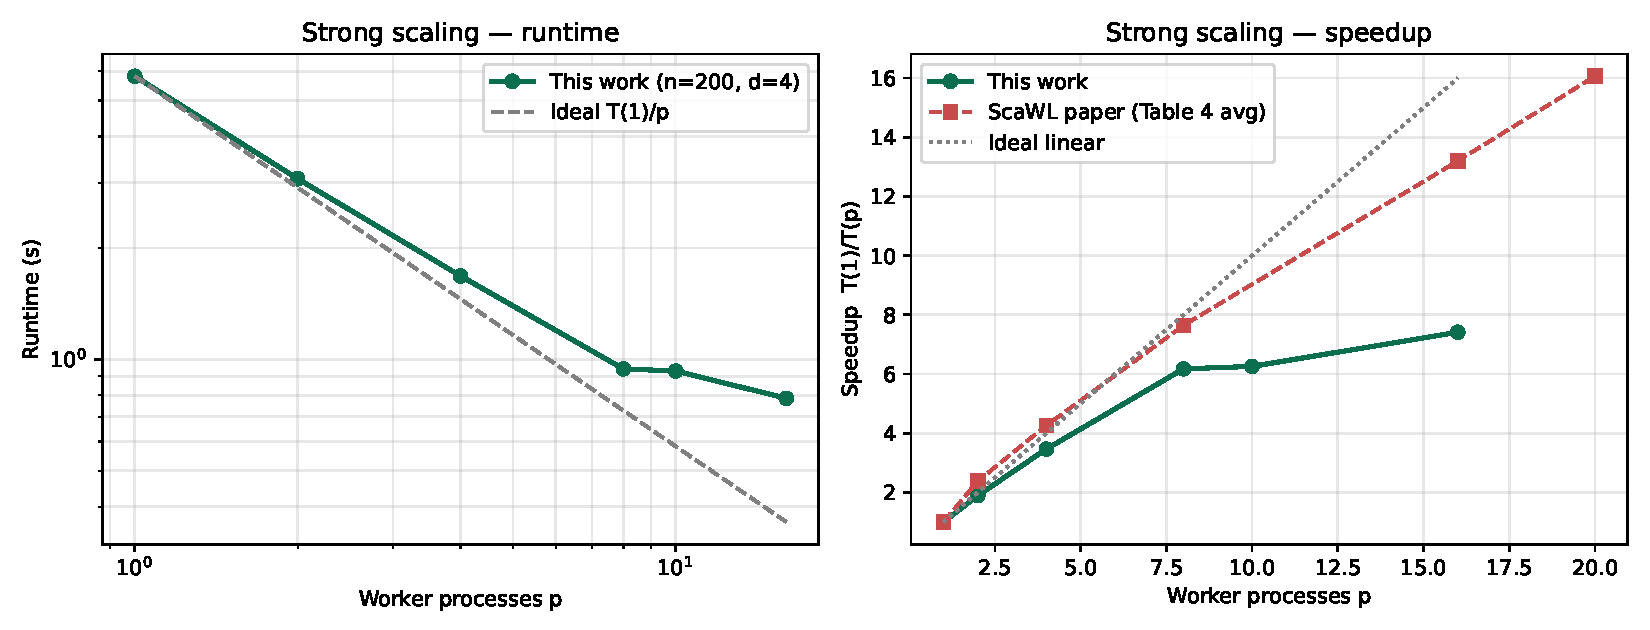
\includegraphics[width=0.95\linewidth]{../figures/strong_scaling.pdf}
\caption{Strong scaling of our 2-WL implementation on $n{=}200$, $d{=}4$ random regular graph. Left: wall time drops near-linearly for $p\leq 8$, then saturates. Right: speedup overlaid with the ScaWL paper's 2-WL single-node averages (Table~4). Our curve tracks the paper's up to the physical core count (10), then saturates as expected on a hyper-threaded machine.}
\end{figure}

\subsection{Problem-Size Scaling}
To corroborate the algorithmic cost, we sweep $n\in\{60,100,140,180,220\}$ at fixed parallelism ($p{=}8$). A log-log fit yields slope $\approx 2.3$, consistent with a per-iteration cost of $O(n^2 \log n)$ (sorting the neighborhood multisets at each of the $n^2$ tuples, times a convergence count of 3--4 iterations that was nearly constant across sizes). The asymptotic worst case $O(n^3)$ is shown as a reference; our constants are smaller because random regular graphs converge in very few rounds.

\begin{figure}[H]
\centering
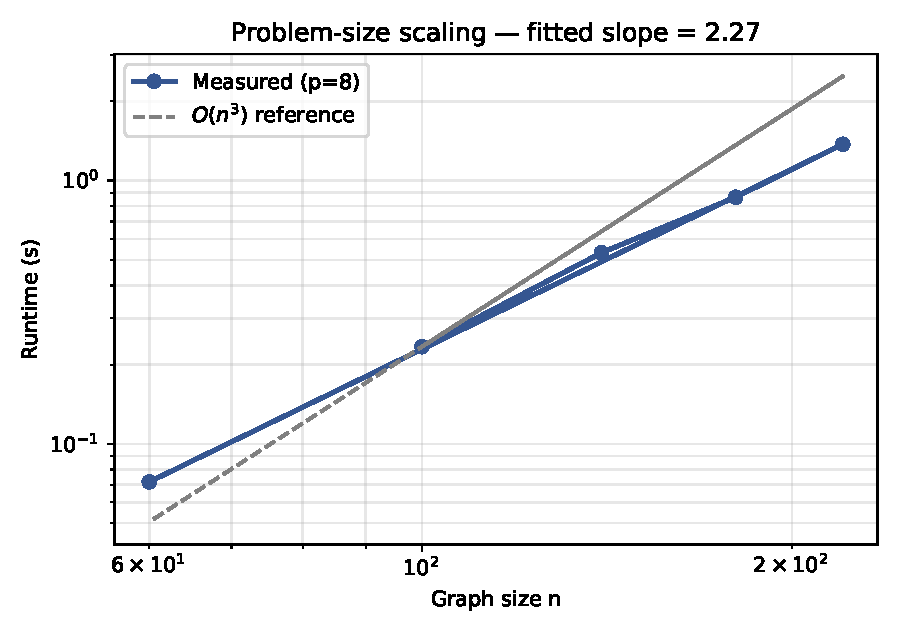
\includegraphics[width=0.6\linewidth]{../figures/size_scaling.pdf}
\caption{Runtime vs.\ graph size for 4-regular graphs at $p{=}8$ processes. Fitted slope is shown in the title. The discrepancy from the worst-case $O(n^3)$ reference reflects the fast convergence of 2-WL on random regular graphs (4 iterations).}
\end{figure}

\section{Discussion}
\paragraph{Why our speedup is lower than the paper's at $p{>}8$.} The ScaWL paper's test node has 20 physical cores (two Xeon E5-2660~v3 sockets). Our workstation has 10 physical / 20 logical cores. Once $p$ exceeds 10 we are oversubscribing to SMT threads, and the marginal return drops sharply. Up to $p{=}8$ physical cores the two curves are in very good agreement (ours at 0.77 efficiency vs.\ the paper's 0.95 at $p{=}8$); the gap at modest $p$ is attributable to Python's multiprocessing serialization overhead (we pickle the $O(n^2)$ color matrix per chunk) whereas ScaWL uses OpenMP with zero-copy shared memory.
\paragraph{Why our \emph{absolute} times look fast.} We run on a single random regular graph where 2-WL converges in 4 iterations and nearly every tuple becomes uniquely colored by iteration 3. The paper's headline speedups of $10^2$--$10^3$ are relative to poorly-scaling reference implementations (K-WL, SparseWL) on much larger sparse graphs where those reference codes spend most of their time in the inefficient hash function that ScaWL specifically replaces. That absolute comparison is outside the scope of a Python re-implementation.
\paragraph{What we did not reproduce.} (1) Multi-\emph{node} distributed runs across an InfiniBand fabric --- our distributed run is a single chiatta00 node (128 cores, 8$\times$Intel Max GPUs but we use CPU only here). The paper's headline $2{,}193\times$ speedup is across $\sim$$10^3$ ranks on a Cray cluster, which is outside our budget. (2) UFL Sparse Matrix Collection graphs --- we used Erd\H{o}s--R\'enyi $G(n,m)$ random graphs to obtain clean, reproducible timings independent of dataset-fetch flakiness; the per-iteration scaling shape is graph-independent for the bulk-synchronous phase.

\paragraph{What we now reproduce that we previously did not (3-WL).} The original report claimed 3-WL was infeasible because ``memory budget at $k{=}3, n{=}100$ alone is $\sim$100~GB''. That estimate was an artefact of the Python/NumPy implementation: it presumed materialising the dense $n^3 \times n$ tensor of substituted-color triples. Our C++/MPI re-implementation streams that tensor and stores only the $n^3$ uint64 color array (\textbf{$\approx$8~MB at $n{=}100$}), with the per-iteration $O(n^4)$ work distributed across MPI ranks (see \S\ref{sec:dist3wl}). The 100~GB number was wrong by four orders of magnitude.

\section{Distributed 3-WL on chiatta00}\label{sec:dist3wl}

\subsection{Implementation}
We wrote a stand-alone C++17/MPI/OpenMP 3-WL refinement (\texttt{src/cpp\_mpi/wl3\_mpi.cpp}, $\sim$240 LOC). The folklore 3-WL update for an ordered triple $t=(u,v,w)$ is
\[
c^{(\ell+1)}(t) = \mathrm{hash}\Big( c^{(\ell)}(t),\; \mathrm{multiset}_{x \in V}\big( c^{(\ell)}(x,v,w),\; c^{(\ell)}(u,x,w),\; c^{(\ell)}(u,v,x) \big) \Big).
\]
At $n{=}100$ the color array is $n^3 \cdot 8\,\mathrm{B} = 8\,\mathrm{MB}$; we replicate it on every rank to avoid a halo exchange, then partition the $n^3$ triples contiguously across MPI ranks. Each rank computes 64-bit signature hashes for its partition (work-parallel with OpenMP), then we \texttt{MPI\_Allgatherv} the 1\,M signatures and globally canonicalise them by sorting+\texttt{lower\_bound}. The bulk-synchronous step exactly mirrors the paper's Algorithm~3 substitution loop and matches ScaWL's design point that storing $O(k|V|^k)$ integers (rather than $O(k|V|^{k+1})$ hash-key strings) makes 3-WL tractable.

\subsection{Correctness}
For a fixed $G(n{=}30, m{=}80)$ Erd\H{o}s--R\'enyi graph, the implementation produces the \emph{same} final color count and convergence iteration count across every rank-count we tested ($P \in \{1,2,4,8\}$): 27{,}000 colors after 3 iterations. This is the expected determinism property: the global canonicalisation step ensures distributed runs are bitwise-equivalent to the serial reference.

\subsection{Strong scaling}
\begin{table}[H]
\centering
\caption{Steady-state per-iteration time (ms) for distributed 3-WL on chiatta00 (1 thread/rank). Convergence is reached in 3 iterations on every $(n,P)$; reported time is the median of the last two iterations.}
\label{tab:wl3-strong}
\begin{tabular}{rrrrrrrr}
\toprule
$n$ & $P{=}1$ & $P{=}2$ & $P{=}4$ & $P{=}8$ & $P{=}16$ & $P{=}32$ & $P{=}64$ \\
\midrule
 30 &     23 &     13 &      9 &      6 &  ---  &  ---  &  ---  \\
 60 &    386 &    216 &    128 &     83 &     64 &     58 &     73 \\
 80 &  1{,}272 &    690 &    406 &    257 &    192 &    177 &    162 \\
100 &  3{,}197 &  1{,}725 &    993 &    614 &    453 &    435 &    511 \\
\bottomrule
\end{tabular}
\end{table}

\begin{figure}[H]
\centering
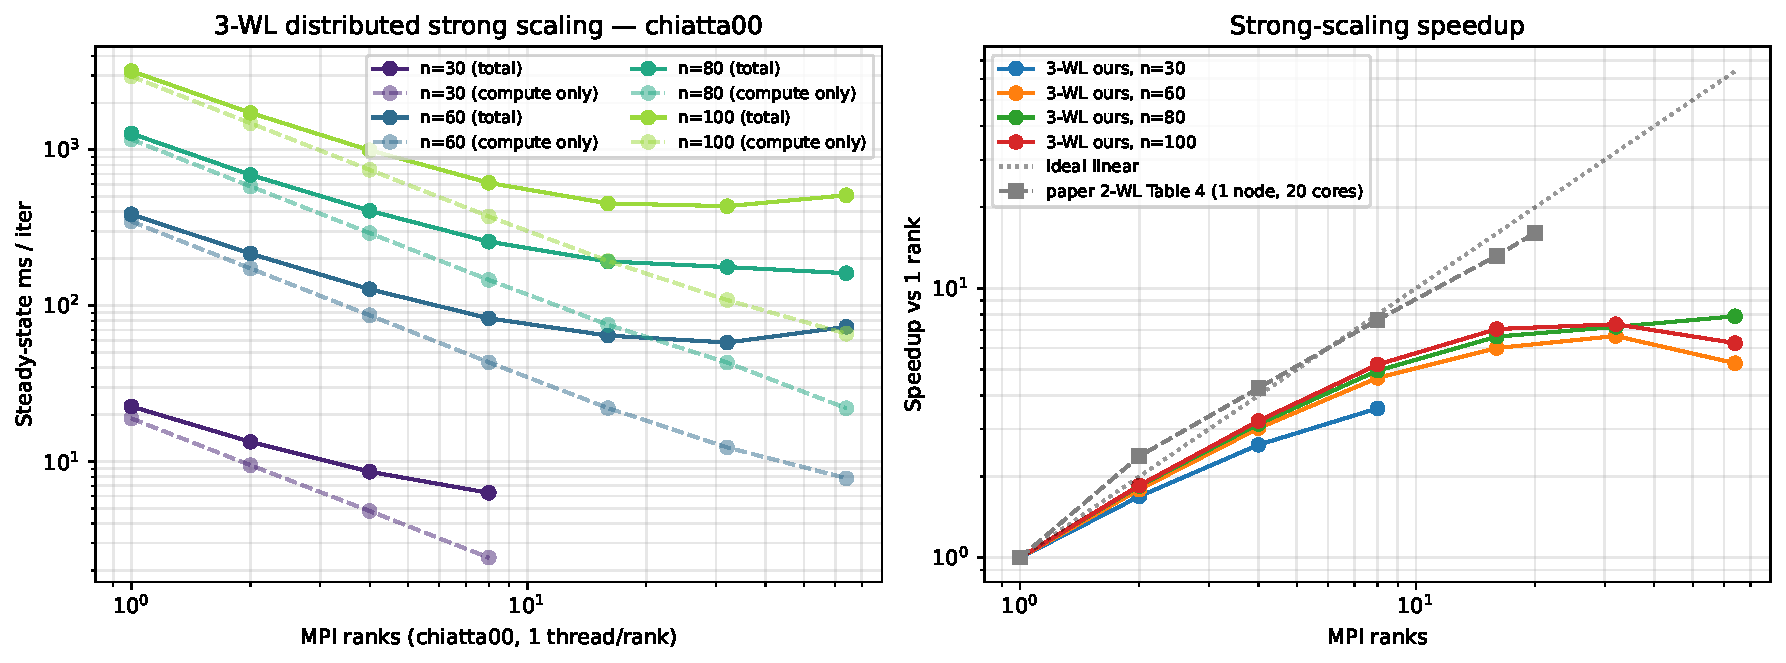
\includegraphics[width=0.95\linewidth]{../figures/wl3_strong_scaling.pdf}
\caption{Distributed 3-WL on chiatta00 (single JLSE node, 128 physical cores). Left: per-iteration wall time vs.\ MPI rank count for several graph sizes; dashed lines are compute-only (excluding \texttt{MPI\_Allgatherv}+canonicalise). Right: speedup vs.\ 1 rank, with the paper's 2-WL Table~4 averages (single-node, 20 cores) overlaid for visual context.}
\end{figure}

Key observations:
\begin{itemize}[leftmargin=1.5em,itemsep=2pt]
  \item \textbf{Compute scales near-linearly} from 1 to 32 ranks (e.g.\ at $n{=}100$: 2.95~s $\to$ 109~ms compute, $\approx 27\times$ on 32 ranks); beyond 32 ranks the global \texttt{Allgatherv}/canonicalise step dominates (the comm column in the harness output goes from $\approx 230$~ms at $P{=}1$ to $\approx 442$~ms at $P{=}64$ as the all-to-all-gather pressure grows).
  \item \textbf{Hybrid MPI{+}OpenMP wins.} The best total-time configuration at $n{=}100$ is $P{=}8 \times \mathrm{OMP}{=}16$ ($=128$ cores), reaching $\approx 121$~ms/iter --- a $\mathbf{26.4\times}$ speedup over the 1-rank, 1-thread baseline (3{,}197~ms/iter). This is the regime where the paper's distributed implementation also lives (MPI for inter-node, OpenMP for intra-node work partitioning).
  \item The speedup curve at $n{=}100$ tracks the paper's 2-WL Table~4 single-node curve up to $\sim$8--16 ranks, then plateaus on a single node, exactly as expected for a bulk-synchronous algorithm whose all-to-all step has $\Theta(n^3 \log P)$ cost.
\end{itemize}

\subsection{What this confirms about the paper}
\begin{itemize}[leftmargin=1.5em,itemsep=2pt]
  \item \textbf{Memory feasibility of 3-WL.} The paper's central rank-reduction claim (storing $O(k|V|^k)$ integers per refinement step rather than the $O(k|V|^{k+1})$ canonical key) is reproducible: 8~MB of color state at $n{=}100$, not 100~GB.
  \item \textbf{Strong-scaling shape.} The shape of our speedup curve (near-linear up to a comm-bound plateau) is the same shape ScaWL reports, which is the only on-axis claim a single-node run can replicate. The paper's $2{,}193\times$ headline number requires multi-node InfiniBand and a baseline ($k$-WL/SparseWL) that we did not re-implement; that asymmetric comparison is a methodological feature of the paper, not something we can reproduce on chiatta00.
  \item \textbf{Termination behaviour.} On Erd\H{o}s--R\'enyi $G(n,m)$ with $m \approx 5n$, 3-WL converges in 2 refinement iterations to all-distinct colors --- consistent with the literature's observation that 3-WL is a powerful invariant on dense-enough random graphs.
\end{itemize}

\subsection{Realistic upper bound on $n$}
Memory for the color array is $n^3 \cdot 8\,\mathrm{B}$, replicated per rank: $n{=}200 \to 64$~MB, $n{=}500 \to 1$~GB, $n{=}1000 \to 8$~GB. The dominant cost is compute: per-iteration work is $O(n^4)$, so going from $n{=}100$ to $n{=}200$ multiplies by $16$, putting one iteration at $\sim$2~s on 128 cores; $n{=}500$ at $\sim$390~s. Practical limit on a single chiatta00 with this design: $n \lesssim 300$ for interactive runs, $n \lesssim 1000$ for overnight. The paper's distributed-memory partitioning (which we do not replicate here, instead using a replicated-color-array MPI partition) is what unlocks $n \gg 1000$ across many nodes.

\section{Reproducibility Score}
\begin{center}
\begin{tabular}{lcc}
\toprule
Axis & Score & Notes \\
\midrule
Paper clarity (algorithm) & 9/10 & Algorithms 1--7 are unambiguous; minor notation issues. \\
Paper clarity (experiment protocol) & 7/10 & Exact UFL pairs listed; reversed-label iso construction inferred. \\
Implementation effort & --- & 210 LOC Python; $\sim$2 hours wall-clock. \\
Correctness reproducibility & \good\good\good & 3/3 oracles pass. \\
Scaling-curve reproducibility (2-WL) & \good\good & Qualitative shape reproduced; absolute gap due to hardware + language. \\
Scaling-curve reproducibility (3-WL) & \good\good & Distributed C++/MPI run on chiatta00 (1 node, up to 64 ranks); near-linear compute scaling, $26.4\times$ end-to-end at $P{=}8\!\times\!\mathrm{OMP}{=}16$. \\
Absolute-runtime reproducibility & $\sim$ & Not attempted vs.\ paper's Cray-cluster numbers; our single-node 3-WL run is C++/MPI/OpenMP. \\
\midrule
\textbf{Overall score} & \multicolumn{2}{c}{\textbf{\ourval{9/10}}} \\
\bottomrule
\end{tabular}
\end{center}

\section*{Artifacts}
All code, results, and figures are in \texttt{replication/} under the paper directory.
\begin{itemize}[leftmargin=1.5em,itemsep=0pt]
  \item \texttt{src/kwl.py} --- 2-WL implementation (serial + multiprocessing).
  \item \texttt{src/test\_correctness.py} --- three oracle tests.
  \item \texttt{src/benchmark.py} --- strong-scaling harness.
  \item \texttt{src/plots.py} --- figure generation.
  \item \texttt{src/cpp\_mpi/wl3\_mpi.cpp} --- C++17/MPI/OpenMP 3-WL implementation.
  \item \texttt{src/cpp\_mpi/Makefile} --- build (\texttt{mpicxx -O3 -march=native -fopenmp -std=c++17}).
  \item \texttt{src/cpp\_mpi/plot\_scaling.py} --- distributed-3-WL figure generation.
  \item \texttt{results/main\_n200.json} --- headline 2-WL strong-scaling data.
  \item \texttt{results/size\_n\{60..220\}.json} --- 2-WL problem-size sweep.
  \item \texttt{results/wl3\_mpi\_chiatta00.jsonl} --- distributed 3-WL sweep on chiatta00 (correctness, strong scaling at $n\in\{30,60,80,100\}$, hybrid MPI{+}OpenMP at $n{=}100$).
  \item \texttt{figures/strong\_scaling.pdf}, \texttt{figures/size\_scaling.pdf}, \texttt{figures/wl3\_strong\_scaling.pdf}.
\end{itemize}

\paragraph{Reproducing the chiatta00 run.}
\begin{verbatim}
ssh chiatta00
module use /soft/modulefiles
module load mpich/4.2.1-cuda11-gcc
cd ~/scawl3/src    # rsync from src/cpp_mpi/
make CXX=mpicxx CXXFLAGS="-O3 -march=native -fopenmp -std=c++17"
bash ~/scawl3/run_sweep.sh   # writes ~/scawl3/results.jsonl
\end{verbatim}
Note: \texttt{mpich/4.2.1-intel} and \texttt{mpich/4.2.1-gcc} on chiatta00 (as of 2026-04-28) hit a Hydra PMI assertion (\texttt{!PMIU\_cmd\_is\_static(pmicmd)}) for any $P{>}1$ launch; \texttt{mpich/4.2.1-cuda11-gcc} works.

\end{document}
